% !TEX root = ../../rl_book.tex
\section{Probability}
\label{sec:probability}

We cover probability with a light touch on measure theory; these notes were prepared while following the lecture series Probability Foundations for Electrical Engineers (IIT M).

\subsection{Introduction}

Probability is the science of randomness that seeks to quantify patterns underlying seemingly non-deterministic events. Andrey Kolmogorov is regarded as the father of modern probability theory. We study probability rigorously because intuitive reasoning can often lead to paradoxes. A famous example is Bertrand’s paradox, where different definitions of “randomness” lead to different probability values. The problem is stated as follows: A chord is drawn at random in a circle. What is the probability that the chord is longer than the side of the equilateral triangle inscribed in the circle? This paradox arises because the sample space is continuous (infinite) and must therefore be defined carefully to avoid ambiguity.

\subsection{Cardinality and Countability}

\subsubsection{Functions and Mappings.}
Given two sets \( A \) and \( B \), a \emph{function} \( f: A \to B \) is a rule that associates every element of \( A \) with a unique element of \( B \).  
The set \( A \) is called the \emph{domain}, and the set \( B \) is called the \emph{codomain}.  
The \emph{range} (or image) of \( f \) is the subset of \( B \) consisting of all elements that are actually mapped to by elements of \( A \), i.e.,
\[
\mathrm{Range}(f) = \{\, f(a) \mid a \in A \,\} \subseteq B.
\]
Note that every element of \( A \) must be mapped to exactly one element of \( B \), although some elements of \( B \) may not receive a mapping from \( A \).

\paragraph{Injective (One-to-One) Function.}
A function \( f: A \to B \) is said to be \emph{injective} if distinct elements of \( A \) map to distinct elements of \( B \). Formally,
\[
f(a_1) = f(a_2) \implies a_1 = a_2, \quad \forall a_1, a_2 \in A.
\]
Equivalently, every element of the range \( \mathrm{Range}(f) \subseteq B \) has a unique preimage in \( A \).

\paragraph{Surjective (Onto) Function.}
A function \( f: A \to B \) is \emph{surjective} if every element of the codomain \( B \) has at least one preimage in \( A \); that is,
\[
\forall b \in B, \; \exists a \in A \text{ such that } f(a) = b.
\]
Hence, for a surjective function, the range equals the codomain: \( \mathrm{Range}(f) = B \).

\paragraph{Bijective Function.}
A function \( f: A \to B \) is \emph{bijective} if it is both injective and surjective.  
In this case, each element of \( B \) has exactly one preimage in \( A \), and \( f \) is said to be \emph{invertible}.  
Its inverse \( f^{-1}: B \to A \) is also a well-defined function satisfying
\[
f^{-1}(f(a)) = a, \quad \forall a \in A, \qquad \text{and} \qquad f(f^{-1}(b)) = b, \quad \forall b \in B.
\]


\subsubsection{Cardinality}

Cardinality is a measure of the ``size'' or number of elements in a set. For finite sets, this is simply the number of elements. However, comparing the sizes of infinite sets is more subtle. For instance, both the set of natural numbers $\mathbb{N}$ and the set of real numbers $\mathbb{R}$ are infinite, yet they are not of the same size. How, then, can we compare their sizes?

\paragraph{Cantor's Argument.}
Two sets have the same cardinality if there exists a bijective (one-to-one and onto) function between them.

\paragraph{Definition.}
Let $A$ and $B$ be two sets.
\begin{enumerate}
    \item $A$ and $B$ are said to have the same cardinality, denoted $|A| = |B|$, if there exists a bijective function $f: A \to B$.
    \item If there exists an injective (one-to-one) function $f: A \to B$ but no bijection, then $B$ has greater or equal cardinality, i.e., $|B| \geq |A|$.
    \item If there exists an injective but not surjective function $f: A \to B$, then $|B| > |A|$.
\end{enumerate}

\paragraph{Theorem.}
The cardinality of the real numbers $\mathbb{R}$ is strictly greater than that of the natural numbers $\mathbb{N}$.

\paragraph{Proof Sketch.}
(Using Cantor's diagonal argument (the ideas to construct new real number by flipping the diagonal entry which will be different from all existing entries).)  
Assume, for contradiction, that there exists a bijection $f: \mathbb{N} \to (0,1) \subset \mathbb{R}$, meaning every real number in $(0,1)$ can be written as a decimal expansion and listed as $f(1), f(2), f(3), \dots$.  
Construct a new real number $r$ by altering the $n$-th digit of $f(n)$ (for instance, replace the $n$-th digit by $5$ if it is not $5$, otherwise by $4$). By construction, $r$ differs from every $f(n)$ in at least one digit, so $r$ is not in the list.  
This contradicts the assumption that $f$ is surjective. Therefore, no bijection exists, and we conclude that
\[
|\mathbb{R}| > |\mathbb{N}|.
\]
Hence, the set of real numbers is uncountably infinite, while the set of natural numbers is countably infinite.


\subsubsection{Countability}

\paragraph{Definition.}
\begin{itemize}
    \item A set $E$ is said to be \textbf{countably infinite} if it is equi-cardinal with $\mathbb{N}$, i.e., there exists a bijection between $E$ and $\mathbb{N}$.
    \item A set is said to be \textbf{countable} if it is either finite or countably infinite.
\end{itemize}

\noindent\textbf{Examples.}
\begin{itemize}
    \item The set of even numbers is equi-cardinal with $\mathbb{N}$ (via $f(n) = 2n$).
    \item The set of integers $\mathbb{Z}$ is countably infinite (we can enumerate them as $0, 1, -1, 2, -2, \ldots$).
    \item The set of rational numbers $\mathbb{Q}$ is also countably infinite.
\end{itemize}

\paragraph{Theorem.}
The set of rational numbers $\mathbb{Q}$ is countably infinite.

\paragraph{Proof Sketch.}
Every rational number can be written as a fraction $\frac{p}{q}$ where $p \in \mathbb{Z}$ and $q \in \mathbb{N}$.  
We can list all such pairs $(p, q)$ in a two-dimensional grid indexed by integers $p$ and positive integers $q$.  
By enumerating these pairs in a diagonal manner (e.g., by increasing $|p| + q$) and skipping equivalent fractions (such as $\frac{1}{2}$ and $\frac{2}{4}$), we can construct a sequence that lists all rational numbers exactly once.  
Thus, there exists a bijection between $\mathbb{Q}$ and $\mathbb{N}$, implying that $\mathbb{Q}$ is countably infinite.  
\[
|\mathbb{Q}| = |\mathbb{N}|.
\]

\paragraph{Note.}
Uncountable sets (such as $\mathbb{R}$) are ``larger'' infinities than $\mathbb{N}$.

\paragraph{Theorem.}
Let $I$ be a countable index set, and let $\{A_i : i \in I\}$ be a collection of countable sets.  
Then the union $\displaystyle \bigcup_{i \in I} A_i$ is countable.  
In other words, a countable union of countable sets is countable.

\paragraph{Proof Sketch.}
For each $i \in I$, enumerate the elements of $A_i$ as $A_i = \{a_{i1}, a_{i2}, a_{i3}, \ldots\}$.  
Arrange these elements in a two-dimensional grid with rows indexed by $i$ and columns by $j$.  
Since both $I$ and each $A_i$ are countable, the set of all pairs $(i,j)$ is countable (using the same diagonal argument as before).  
Now define a mapping from $\mathbb{N}$ to $\bigcup_{i \in I} A_i$ by traversing this grid diagonally and listing each $a_{ij}$ encountered.  
This provides an enumeration of the entire union, proving that
\[
\Big|\bigcup_{i \in I} A_i\Big| = |\mathbb{N}|.
\]
Hence, the countable union of countable sets is countable.

\paragraph{Examples of Countable Sets}
\begin{enumerate}
    \item \textbf{Algebraic Numbers:} The set of all real numbers that are roots of polynomials with integer coefficients. Since each polynomial has finitely many roots, and there are countably many such polynomials, the set of algebraic numbers is countable.
    \item \textbf{Computable Numbers:} The set of all real numbers that can be computed to any desired degree of precision by a terminating algorithm or program. As there are only countably many possible programs, this set is also countable.
\end{enumerate}

\subsubsection{Uncountable Sets}

\paragraph{Definition.}
A set $F$ is said to be \textbf{uncountable} if it has cardinality strictly greater than that of $\mathbb{N}$, i.e., $|F| > |\mathbb{N}|$.  
Equivalently, there exists an injective (one-to-one) mapping from $\mathbb{N}$ to $F$, but no bijection between them.

\paragraph{Examples.}
\begin{itemize}
    \item The set of real numbers $\mathbb{R}$.
    \item The set of irrational numbers $\mathbb{R} \setminus \mathbb{Q}$.
    \item The set of all infinite binary strings $\{0,1\}^{\infty}$.
    \item The power set of the natural numbers $\mathcal{P}(\mathbb{N})$.
\end{itemize}

\paragraph{Theorem.}
The set $\{0,1\}^{\infty}$ of all infinite binary strings is uncountable.

\paragraph{Proof Sketch.}
(Sketch via Cantor’s diagonal argument.)  
Assume that $\{0,1\}^{\infty}$ is countable. Then all binary strings can be listed as:
\[
s_1, s_2, s_3, \ldots
\]
where each $s_i = (s_{i1}, s_{i2}, s_{i3}, \ldots)$ is an infinite sequence of $0$s and $1$s.  
Construct a new binary string $t = (t_1, t_2, t_3, \ldots)$ by flipping the $i$-th digit of $s_i$, i.e.,
\[
t_i = 
\begin{cases}
0, & \text{if } s_{ii} = 1, \\
1, & \text{if } s_{ii} = 0.
\end{cases}
\]
By construction, $t$ differs from each $s_i$ in at least one position (the $i$-th).  
Hence, $t$ is not in the list, contradicting the assumption that the set is countable.  
Therefore, $\{0,1\}^{\infty}$ is uncountable.

\paragraph{Remark.}
To show that another set $A$ is uncountable, it suffices to construct an injective (or bijective) mapping from $\{0,1\}^{\infty}$ to $A$.  
For instance, the interval $[0,1]$ is uncountable because each real number in $[0,1]$ can be represented as an infinite binary sequence.


\subsection{Probability Spaces}

\subsubsection{Random Experiment and Sample Space}

\paragraph{Definition.}
A \textbf{random experiment} is a process that leads to one of several possible outcomes, where the outcome cannot be predicted with certainty in advance.

\paragraph{Sample Space.}
The \textbf{sample space} $S$ (also denoted $\Omega$) is the set of all possible outcomes of a random experiment that we are interested in:
\[
S = \{\text{all possible outcomes}\}.
\]

\paragraph{Example.}
\begin{itemize}
    \item Fair coin toss: coin faces or number of tumbles in air
    \item Velocity with which the coin strikes the ground $\mathbb{R}^+$
\end{itemize}

\paragraph{Remark.}
The definition of $S$ depends on the level of detail we are interested in.
For example, if we include physical parameters of a coin toss (e.g., velocity, angle, or spin), then $S$ may be uncountable. An outcome is denoted by $w \in S$.

\begin{center}
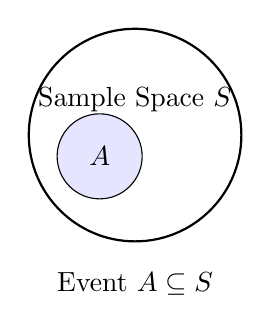
\begin{tikzpicture}[scale=0.9]
\draw[thick] (0,0) circle (1.5);
\node at (0,0.5) {Sample Space $S$};
\draw[fill=blue!10] (-0.5,-0.3) circle (0.6);
\node at (-0.5,-0.3) {$A$};
\node[below] at (0,-1.8) {Event $A \subseteq S$};
\end{tikzpicture}
\end{center}



\subsubsection{Events}

\paragraph{Definition.}
An \textbf{event} is any subset of the sample space $S$ which are of intereset.  
An event occurs if the outcome of the experiment belongs to that subset.

\paragraph{Example.}
When tossing two coins:
\[
S = \{HH, HT, TH, TT\}.
\]
Let $A =$ ``at least one head'' $\Rightarrow A = \{HH, HT, TH\}$.

\paragraph{Note.}
\begin{itemize}
    \item Not all subsets of $S$ are necessarily events (especially in uncountable $S$).
    \item Every event is a subset of $S$.
    \item In uncountable spaces, only measurable subsets are valid events.
    \item some subsets don't behave nicely, so we study it from the lens of measurable space.
\end{itemize}


\subsubsection{Algebra and $\sigma$-Algebra of Events}

\paragraph{Algebra of Sets.}
A collection $\mathcal{F}_0$ of subsets of $S$ is called an \textbf{algebra} if:
\begin{enumerate}
    \item $S \in \mathcal{F}_0$,
    \item If $A \in \mathcal{F}_0$, then $A^c \in \mathcal{F}_0$,
    \item If $A_1, A_2 \in \mathcal{F}_0$, then $A_1 \cup A_2 \in \mathcal{F}_0$.
\end{enumerate}
That is, $\mathcal{F}_0$ is closed under complement and finite unions.

\paragraph{Example.}
Consider tossing a coin until the first head appears.  
Then $S = \{H, TH, TTH, TTTH, \ldots\}$, which is countably infinite.  
The algebra $\mathcal{F}_0$ does not necessarily include infinite unions of its sets.

\paragraph{$\sigma$-Algebra.}
A collection $\mathcal{F}$ of subsets of $S$ is called a \textbf{$\sigma$-algebra} if:
\begin{enumerate}
    \item $S \in \mathcal{F}$,
    \item If $A \in \mathcal{F}$, then $A^c \in \mathcal{F}$,
    \item If $\{A_i\}_{i=1}^\infty \subseteq \mathcal{F}$, then $\bigcup_{i=1}^\infty A_i \in \mathcal{F}$.
\end{enumerate}

\paragraph{Note.}
Every $\sigma$-algebra is also an algebra, but the converse is not true. $\mathcal{F}$ is basically a subset of power-set of $S$.

\noindent
The cardinality of $\mathcal{F}$ could be uncountable, it's matter of how big the uncountable is eg. $2^\mathbb{N}$ vs $2^\mathbb{R}$.



\subsubsection{Measure and Probability Measure}

\paragraph{Measurable Sets.}
Subsets belonging to $\mathcal{F}$ are called \textbf{$\mathcal{F}$-measurable sets}.  
The pair $(S, \mathcal{F})$ is called a \textbf{measurable space}. It is not possile to assing probability to all subsets of power set (with uncountable sample space).

\paragraph{Measure.}
A \textbf{measure} is a function
\[
\mu: \mathcal{F} \to [0, \infty]
\]
that satisfies:
\begin{enumerate}
    \item $\mu(\emptyset) = 0$,
    \item For any countable collection of disjoint sets $\{A_i\}$ in $\mathcal{F}$,
    \[
    \mu\left(\bigcup_{i=1}^\infty A_i\right) = \sum_{i=1}^\infty \mu(A_i).
    \]
\end{enumerate}

The triple $(S, \mathcal{F}, \mu)$ is called a \textbf{measure space}. Space is actualy a set with additional structure.

\paragraph{Types of Measures.}
\begin{itemize}
    \item \textbf{Finite measure:} $\mu(S) < \infty$.
    \item \textbf{Infinite measure:} $\mu(S) = \infty$.
    \item \textbf{Probability measure:} $\mu(S) = 1$.
\end{itemize}


\subsubsection{Probability Measure}

A \textbf{probability measure} $P$ on $(S, \mathcal{F})$ is a function
\[
P: \mathcal{F} \to [0, 1]
\]
such that:
\begin{enumerate}
    \item $P(\emptyset) = 0$,
    \item $P(S) = 1$,
    \item For any countable disjoint collection $\{A_i\} \subseteq \mathcal{F}$,
    \[
    P\left(\bigcup_{i=1}^\infty A_i\right) = \sum_{i=1}^\infty P(A_i).
    \] The summation is monotonically non-decreasing so the sum always converges.
\end{enumerate}

Then $(S, \mathcal{F}, P)$ is called a \textbf{probability space}.  
Elements of $\mathcal{F}$ are the measurable events.

\paragraph{Note.} $\mathcal{F}$ has smaller or equal cardinality than that of power set of $S$. \textbf{Basically, to study probability with nice collection of events.}

\subsubsection{Properties of Probability Measure}

For any events $A, B \in \mathcal{F}$:
\begin{enumerate}
    \item $P(A^c) = 1 - P(A)$
    \item If $A \subseteq B$, then $P(A) \leq P(B)$ (Monotonicity)
    \item $P(A \cup B) = P(A) + P(B) - P(A \cap B)$
    \item Inclusion–Exclusion Principle. For events $A_1, \ldots, A_n$,
\[
P\left(\bigcup_{i=1}^n A_i\right)
= \sum_i P(A_i)
- \sum_{i<j} P(A_i \cap A_j)
+ \sum_{i<j<k} P(A_i \cap A_j \cap A_k) - \cdots
\]
   \item \textbf{Continuity of Probability.} 
    Let $\{A_n\}_{n=1}^\infty \subseteq \mathcal{F}$ be events . Then
    \[
    P\!\left(\bigcup_{n=1}^{\infty} A_n\right) = \lim_{n \to \infty} P(\bigcup_{n=1}^{n} A_n).
    \]
    
    \textbf{Proof Sketch.} 
    Define disjoint sets $B_1 = A_1$, and for $n \ge 2$ let 
    \[
    B_n = A_n \setminus A_{n-1}.
    \]
    Then, $\{B_n\}$ are pairwise disjoint and 
    \[
    \bigcup_{n=1}^{\infty} A_n = \bigcup_{n=1}^{\infty} B_n.
    \]
    By countable additivity,
    \[
    P\!\left(\bigcup_{n=1}^{m} B_n\right) = \sum_{i=1}^{m} P(B_i).
    \]
    Taking the limit as $m \to \infty$ and using monotone convergence,
    \[
    P\!\left(\bigcup_{n=1}^{\infty} A_n\right) 
    = \lim_{m \to \infty} \sum_{i=1}^{m} P(B_i).
    \]
    Thus, the probability measure $P$ is \emph{continuous from below}. 
    Moving the limit outside the measure illustrates the continuity property of $P$.

    
    \item Continuity of Probability (corollary). If $\{A_n\}$ is an increasing sequence of events ($A_1 \subseteq A_2 \subseteq \cdots$), then
\[
P\left(\bigcup_{n=1}^\infty A_n\right) = \lim_{n \to \infty} P(A_n).
\]

    \item If $\{A_n\}$ is decreasing, then
\[
P\left(\bigcap_{n=1}^\infty A_n\right) = \lim_{n \to \infty} P(A_n).
\]
    \item Union Bound: 
   \[
P\!\left(\bigcup_{n=1}^{\infty} A_n\right)
\leq
\sum_{n=1}^{\infty} P(A_n).
\]

\end{enumerate}

\begin{center}
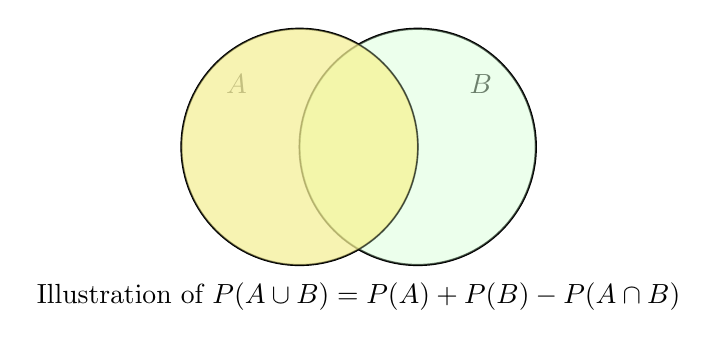
\begin{tikzpicture}[scale=1]
\draw[thick] (0,0) circle (1.5);
\draw[thick] (1.5,0) circle (1.5);
\node at (-0.8,0.8) {$A$};
\node at (2.3,0.8) {$B$};
\node at (0.75,-1.9) {Illustration of $P(A \cup B) = P(A) + P(B) - P(A \cap B)$};
\draw[fill=blue!15, opacity=0.5] (0,0) circle (1.5);
\draw[fill=green!15, opacity=0.5] (1.5,0) circle (1.5);
\draw[fill=yellow!50, opacity=0.6] (0,0) circle (1.5);
\end{tikzpicture}
\end{center}







\subsubsection{Discrete Probability Space}
% Mod 1 Lec 7 https://www.youtube.com/watch?v=PseYlBGV_00&list=PLbMVogVj5nJQqGHrpAloTec_lOKsG-foc&index=7

The discrete space is easy to study since the power set of $S$ contains all measurable sets.
Here, $S$ is countable (finite or countably infinite). Now, we can take set of all events $\mathcal{F}$ as power set $2^{|S|}$ and assign probability to each event. 

If the sample space $S$ is finite or countable, and probabilities are assigned to each outcome $w_i$ such that
\[
P(w_i) \geq 0, \quad \sum_i P(w_i) = 1,
\]
then for any event $A \subseteq S$,
$P(A) = \sum_{w_i \in A} P(\{w_i\})$.
And, $\sum_{w_i \in S} P(w_i) = 1$.

Probabilities are actually assigned to the elements of $\mathcal{F}$ and not to the elements of $S$. However, for discrete case it will be like assigning probability to singleton set ${w} \in \mathcal{F}$. So, $P(w_i)$ is actually $P(\{w_i\})$

How is probability assigned to a singleton set? Since the theory does not prescribe a specific measure for individual singletons, we must determine it empirically through experimentation. Example of assignment if $S=\mathbb{N}$, then $p=1/2^k$ for element $k$ is valid measure (geometric measure). Other measures: Poisson measure.

\subsubsection{Uncountable $S$}

Consider the sample space $S = [0, 1]$, where we imagine throwing a dart uniformly at random onto the line segment. The dart is equally likely to land anywhere between $0$ and $1$, and we wish to assign a **uniform probability measure** on this interval.

However, we cannot assign probabilities to every element of the power set $2^S$. The elementary idea of assigning probabilities to singletons fails in this case: there are uncountably many singleton sets, and summing their probabilities would diverge unless each singleton is assigned probability zero. Moreover, in this continuous setting, we cannot obtain probabilities of intervals simply by adding those of individual points, since the union involved is uncountable.

The key idea is therefore to **abandon the assignment of probabilities to singleton sets** and instead assign probabilities only to more meaningful subsets, such as intervals. The challenge then becomes identifying which subsets should be considered *measurable* and how to assign probabilities to them.

We would like a measure $\mu$ that satisfies the following properties:
\begin{enumerate}
    \item (i) $\mu((a, b)) = \mu([a, b])$, i.e., open and closed intervals have the same measure.
    \item (ii) \textbf{Translation invariance:} $\mu(A) = \mu(A + c)$ for any constant shift $c$, where $A + c = \{x + c : x \in A\}$.
\end{enumerate}

\textbf{Theorem (Impossibility Theorem).}  
There does not exist a measure $\mu(A)$ defined on the full power set $2^S$ (that is, on all subsets of $[0,1]$) satisfying both properties (i) and (ii) for a uniform measure.

Hence, we must **restrict** ourselves to a smaller collection of subsets—those that are still rich enough to include all “interesting” sets like intervals but small enough to admit a consistent measure. This leads to the introduction of the **Borel $\sigma$-algebra**, whose elements, called *Borel sets*, are generated by open intervals through countable unions, intersections, and complements.


\subsection{Generated and Borel $\sigma$-Algebra}

We begin by asking: what should be the smallest $\sigma$-algebra on the real line $\mathbb{R}$?  
We would like to construct a $\sigma$-algebra that contains all intervals and is closed under complementation, countable unions, and intersections.

\paragraph{Generated $\sigma$-Algebra.}
Let $\mathcal{C}$ be an arbitrary collection of subsets of a sample space $S$ (not necessarily a $\sigma$-algebra).  
We aim to construct the smallest $\sigma$-algebra that contains all elements of $\mathcal{C}$.

\begin{definition}[Generated $\sigma$-Algebra]
The \emph{$\sigma$-algebra generated by} $\mathcal{C}$, denoted $\sigma(\mathcal{C})$, is defined as the intersection of all $\sigma$-algebras that contain $\mathcal{C}$:
\[
\sigma(\mathcal{C}) = \bigcap_{\mathcal{F} \supseteq \mathcal{C}} \mathcal{F},
\]
where the intersection is taken over all $\sigma$-algebras $\mathcal{F}$ containing $\mathcal{C}$.
\end{definition}

\begin{theorem}
There exists a smallest $\sigma$-algebra that contains all elements of $\mathcal{C}$.
\end{theorem}

\begin{proof}
Let $\mathfrak{S}$ be the collection of all $\sigma$-algebras that contain $\mathcal{C}$.  
Since the power set $2^S$ is itself a $\sigma$-algebra containing $\mathcal{C}$, the collection $\mathfrak{S}$ is nonempty.  
Define
\[
\sigma(\mathcal{C}) = \bigcap_{\mathcal{F} \in \mathfrak{S}} \mathcal{F}.
\]
The intersection of any family of $\sigma$-algebras is itself a $\sigma$-algebra, hence $\sigma(\mathcal{C})$ is a $\sigma$-algebra that contains $\mathcal{C}$.  
By construction, it is the smallest such $\sigma$-algebra.
\end{proof}

\paragraph{Borel $\sigma$-Algebra.}
If $\mathcal{C}$ is chosen to be the collection of all open intervals in $\mathbb{R}$, then the generated $\sigma$-algebra
\[
\mathcal{B}(\mathbb{R}) = \sigma(\mathcal{C})
\]
is called the \emph{Borel $\sigma$-algebra}.  
It is the smallest $\sigma$-algebra that contains all open intervals of $\mathbb{R}$.  
The sets belonging to $\mathcal{B}(\mathbb{R})$ are called \emph{Borel sets}.



\begin{proposition}
Let $b \in (0,1]$. Then the singleton set $\{b\}$ is a Borel set.
\end{proposition}

\begin{proof}[Proof Sketch]
We can express the singleton $\{b\}$ as a countable intersection of open intervals:
\[
\{b\} = \bigcap_{n=1}^{\infty} (\,b - \tfrac{1}{n},\, b + \tfrac{1}{n}\,).
\]
Since each interval $(b - \tfrac{1}{n},\, b + \tfrac{1}{n})$ is an open set, it belongs to the Borel $\sigma$-algebra.  
Because the Borel $\sigma$-algebra is closed under countable intersections, it follows that $\{b\}$ is a Borel set.
\end{proof}

\paragraph{Examples of Non-Borel Sets.}
While all open, closed, and countable sets are Borel, there also exist subsets of $\mathbb{R}$ that are \emph{not} Borel measurable.  
Famous examples include:
\begin{itemize}
    \item \textbf{Vitali sets} — constructed using the Axiom of Choice by partitioning $\mathbb{R}$ into equivalence classes modulo the rationals.
    \item \textbf{Banach–Tarski paradoxical sets} — subsets of $\mathbb{R}^3$ used in the Banach–Tarski paradox, which demonstrates that certain sets can be decomposed and reassembled into a copy of themselves.
\end{itemize}
These examples highlight the existence of highly non-constructive sets lying outside the Borel $\sigma$-algebra.


\subsubsection{Borel Sets and Lebesgue Measure}

\[
S = (0, 1]
\]
Consider the measure space 
\[
\mathcal{M} = (S, \mathcal{B}),
\]
where $\mathcal{B}$ denotes the Borel $\sigma$-algebra on $S$.  
We aim to define a \emph{uniform measure} on $\mathcal{M}$.

\vspace{0.5em}
\noindent
The intuitive idea is to use \emph{length} as the measure for intervals.  
However, since Borel sets include not only intervals but also more complex (and potentially pathological) subsets, the notion of length must be extended to all elements of $\mathcal{B}$.

\vspace{0.5em}
\noindent
Let $\mathcal{F}_0$ be the collection of all subsets of $S$ that are finite unions of disjoint half-open intervals of the form $(a, b]$, together with the null set.  
For each $A \in \mathcal{F}_0$, we define
\[
\mu(A) = \sum_{i} (b_i - a_i),
\]
where the $(a_i, b_i]$ are the disjoint intervals forming $A$.  
This function $\mu$ represents the intuitive “length” of the set $A$.

\vspace{0.5em}
\noindent
The collection $\mathcal{F}_0$ forms an \emph{algebra} of sets, but it is not a $\sigma$-algebra.  
To obtain a $\sigma$-algebra, we consider
\[
\sigma(\mathcal{F}_0) = \mathcal{B}((0,1]),
\]
the Borel $\sigma$-algebra generated by open (or equivalently half-open) intervals.

\vspace{0.5em}
\noindent
Using the \emph{Carathéodory Extension Theorem}, the measure $\mu$ defined on $\mathcal{F}_0$ can be uniquely extended to a measure on $\mathcal{B}((0,1])$.  
This extended measure is the \emph{Lebesgue measure} restricted to $(0,1]$, and it coincides with our intuitive notion of length on all Borel subsets.

\vspace{0.5em}
\noindent
For example, for any singleton $\{b\} \subseteq (0,1]$, we have
\[
P(\{b\}) = 0,
\]
and for the set of rationals $Q \cap (0,1]$, we also have
\[
P(Q \cap (0,1]) = 0.
\]

\vspace{0.5em}
\noindent
More generally, the Lebesgue measure on $\mathbb{R}$ is denoted by
\[
(\mathbb{R}, \mathcal{B}(\mathbb{R}), \lambda),
\]
where $\lambda$ is infinite and satisfies
\[
\lambda((a,b)) = b - a,
\]
representing the standard notion of length on intervals.
